\documentclass[a4paper,12pt]{article}
% Umlaute im PDF sind nicht zusammengesetzt
\usepackage[T1]{fontenc}
% Umlaute müssen nicht maskiert werden
\usepackage[utf8]{inputenc}
% Titel
\title{Beschwerdemanagement}
% Vektorschriftart
\usepackage{lmodern}
% für Deutsche Begriffe und Silbentrennung
\usepackage[ngerman]{babel}
% Formeln
\usepackage{amsmath}
% Grafiken
\usepackage{graphicx}
% Zeilenabstand 1,5 Zeilen
\usepackage{setspace}
\onehalfspacing
% BibLaTeX benutzen
\usepackage[backend=biber]{biblatex}
\addbibresource{bib/Bibliographie.bib}
% Erlaube Zeilenumbrüche in URLs nach Buchstaben und Zahlen
\setcounter{biburllcpenalty}{7000}
\setcounter{biburlucpenalty}{8000}
\setcounter{biburlnumpenalty}{9000}
% Seitenränder anpassen
\usepackage{geometry}
\geometry{left=2cm, right=2cm, top=2.5cm, bottom=2cm}
% eps-Grafiken
\usepackage{epstopdf}
% Siehe http://tex.stackexchange.com/questions/28198/using-ieeetrantools
\usepackage[retainorgcmds]{IEEEtrantools}
\usepackage{microtype}
% pdf-Metadaten und Hyperlinks
\usepackage[pdfsubject = {{The subject of this thesis}},
pdfkeywords = {{Keyword Keyword2}},
pdfstartview = Fit,
pdfpagelayout = SinglePage,
hidelinks,
pdfusetitle]{hyperref}
% Deutsche Anführungszeichen
\usepackage{csquotes}
%\setcounter{section}{-1}
\begin{document}
	\pagestyle{empty}
	\begin{center}
		
\includegraphics[width=0.35\textwidth]{fig/Logo/h-da-logo-sw.pdf}
		\vfill
		\Large Hochschule Darmstadt \\
		\vspace{12pt}
		Fachbereich Maschinenbau und Kunststofftechnik \normalsize \\
		\vfill
		% \@title und \@author verfügbar machen
		\makeatletter
		\Large\@title \\
		\normalsize
		\vfill
		vorgelegt von \\
		\vspace{12pt}
		\begin{tabular}[h]{lr}
			Dominik Appel & 735399 \\
			Florian Wolfgang Schmitt & 736209 \\
			Fabian Alexander Wilms & 735162 \\
		\end{tabular}
		\makeatother
		\vfill
		Dozent: Prof. Dr. R. Stengler\\
	\end{center}
	\newpage
	\pagestyle{plain}
	\phantomsection
	\addcontentsline{toc}{section}{Inhaltsverzeichnis}
	\tableofcontents
	\newpage
	\phantomsection
	\addcontentsline{toc}{section}{Motivation}
	\section*{Motivation}
	Die Abgasaffäre um den Volkswagenkonzern ist ein aktuelles Thema und immer noch nicht vollständig aufgeklärt. Da die Kunden bis heute noch nicht die Folgen für sich abschätzen können und die Kunden in den USA und Europa zu ihrem Missfallen unterschiedlich behandelt werden, bearbeiten wir, um dies in unserer beruflichen Laufbahn besser zu handhaben, das Thema Beschwerdemanagement.
	\section{Der Beschwerdebegriff}
	\begin{center}
		Definition:
	\end{center}
	\blockquote{Beschwerdemanagement umfasst die Planung, Durchführung und Kontrolle aller Maßnahmen, die ein Unternehmen im Zusammenhang mit Kundenbeschwerden ergreift.} {\cite{Gabler}} \\
	
	Es gibt drei verschiedene Beschwerdearten:
	
	\begin{itemize}
		\item Die Kundenbeschwerde: Der Kunde ist mit der Leistung unzufrieden. \\
		Fallbeispiel: Herr Müller bestellt im Internet ein Smartphone, das erhaltene Smartphone hat nicht die gewünschte Farbe.
		\item Die Lieferantenbeschwerde: Ein Unternehmen ist mit einem Lieferanten unzufrieden. \\
		Fallbeispiel: Ein Automobilhersteller bekommt für die Produktion eine Stahllegierung geliefert. Bei der stichprobenartigen Qualitätskontrolle stellt sich heraus, dass die Stahllegierung nicht die gewünschte Zugfestigkeit besitzt.
		\item Die interne Beschwerde: Das Unternehmen ist vor Auslieferung nicht mit der eigenen Leistung zufrieden. \\
		Fallbeispiel: Ein Hersteller für Servomotoren bemerkt bei der Qualitätsprüfung Ungenauigkeiten in der Position. Es stellt sicher heraus, dass die Zahnräder des Getriebes ein zu großes Spiel aufweisen.
	\end{itemize}\newpage
	\subsection{Unterarten}
	Diese Beschwerdearten lassen sich nach dem Grund der Beschwerde in zwei Unterkategorien aufteilen.
	\begin{itemize}
		\item Produktbeschwerde \\
		Bei der Produktbeschwerde wird die Leistung beanstandet (siehe Fallbeispiele zu Beschwerdearten)
		\item Beschwerde über Kundenbetreuung \\
		Bei der Beschwerde über die Kundenbetreuung ist der Kunde mit dem Service unzufrieden, Beispiele hierfür wären: Zeiten zur Erreichbarkeit, ständig wechselnde Gesprächspartner oder aber auch schlechtes Beschwerdemanagement.
	\end{itemize}
	Innerhalb eines Unternehmens können die Beschwerden weiterhin je nach Auswirkung der Beschwerde zur Kanalisierung unterteilt werden.
	Beispielsweise in Beschwerden über Auswirkungen wie Ausfälle und Defekte und in Beanstandung über schwächere Auswirkungen wie beispielsweise geringe optische Mängel oder den Verdacht auf zukünftige Probleme bei der Produktion.
	\section{Beschwerden als Chance}
	Beschwerden sind Rückmeldungen, welche man als Chance sehen sollte, mit dem Ziel, Gewinn und Wettbewerbsfähigkeit zu erhöhen (vergl. PDCA). Dies vermindert Kundenabwanderung und die erhaltenen Hinweise können im Bezug auf betriebliche Schwächen und Marktchancen ausgewertet werden. \cite{Gabler} Ein Kunde, der sich beschwert, hat die Beziehung zum Unternehmen noch nicht aufgegeben und fühlt sich nach einer erfolgreichen Beschwerdebehandlung enger mit dem Unternehmen verbunden. Zudem kann ein gutes Beschwerdemanagement Kundenbefragungen ersetzen, die kaum weitere Informationen liefern, aber weitere Kosten verursachen. Daher sollte diese Form des Qualitätsmanagements als Weg verstanden werden, der Kosten verhindert anstatt sie zu verursachen. Es lassen sich zwei Teilzielarten ausmachen: Solche, die relevant für die Kundenbeziehung sind und solche, die relevant für die Qualität sind.
	So möchte man gefährdete Kundenbeziehungen stabilisieren, das kundenorientierte Image fördern und so für positive Mundpropaganda sorgen. Außerdem sollte das Feedback genutzt werden, um die Produktqualität zu verbessern. \cite{Gabler}
	\newpage
	\section{Aktives und professionelles Beschwerdemanagement}
	\subsection{Beschwerdemanagement in der Unternehmenspraxis}
	Das Beschwerdemanagement ist in der Norm DIN ISO 10002 definiert, welche seit 2005 gilt. Diese ist zwar eine eigenständige Norm, hängt aber eng mit der DIN ISO 9001 zusammen. Sie enthält begriffliche Festlegungen und Beschreibungen von Prinzipien, zentralen Aufgaben und konkreten Hilfsmitteln des Beschwerdemanagements. Das Beschwerdemanagement gewinnt im Qualitätsmanagement weiterhin immer mehr an Bedeutung. \cite{Gabler, stauss2013beschwerdemanagement} \\
	
	\noindent Möchte man ein Beschwerdemanagement einführen sind wesentliche Änderungen bei den Rahmenfaktoren Personalpolitik, Informationstechnologie und Organisation des Unternehmens nötig.\\
	
	\noindent Um die Annahme von Beschwerden effektiv zu gestalten, müssen die Mitarbeiter in der Beschwerdeannahme, -bearbeitung und -reaktion speziell geschult werden. So sind nicht nur die zwischenmenschlichen Fähigkeiten entscheidend, sondern auch ein fundiertes Wissen über die Produkte und Prozesse des Unternehmens vonnöten, um auf die Beschwerden und Bedürfnisse der Kunden angemessen einzugehen und zu reagieren. Wird dies nicht berücksichtigt, so werden Beschwerden möglicherweise falsch eingeschätzt oder an die falschen Bereiche weitergeleitet.\\
	
	\noindent Die effektive Verwaltung von Beschwerden sollte über EDV-Systeme mit geeigneter Software und Hardware erfolgen, da hier die Beschwerden verwaltet und hierdurch eine einfache Priorisierung, Kategorisierung und Kanalisierung vorgenommen kann. \\
	
	\noindent Auf organisatorischer Seite müssen die Prozesse des Beschwerdemanagements mit geeigneten Schnittstellen, klaren Verantwortlichkeinen, Befugnissen und Hierarchien definiert und in die anderen Prozesse des Unternehmens eingebunden werden. \cite{Gabler}
	
	\subsection{Bausteine des Beschwerdemanagements}
	Die Aufgaben des Beschwerdemanagements lassen sich in acht Bereiche unterteilen, jeweils vier in den Kategorien direktes und indirektes Beschwerdemanagement. Im direkten Beschwerdemanagement steht man im direkten Kontakt mit den Kunden. Dies umfasst Beschwerdestimulierung, Beschwerdeannahme, Beschwerdebearbeitung und Beschwerdereaktion. Im indirekten Beschwerdemanagement gibt es keinen direkten Kundenkontakt, sondern man kümmert sich um Beschwerdeauswertung, Beschwerdemanagement-Controlling, Beschwerdereporting und Beschwerdeinformationsnutzung. \cite{Gabler}
	\begin{figure}[h]
		\begin{center}
			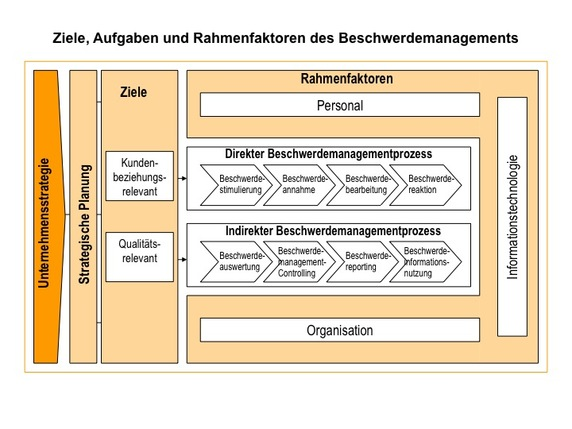
\includegraphics[width=\textwidth]{fig/gabler.jpg}
			\caption{Übersichtsgrafik aus \cite{Gabler}}
		\end{center}
	\end{figure}
	\subsubsection{Direktes Beschwerdemanagement}
	Die Beschwerdestimulierung hat das Ziel, Kunden mit Grund zur Unzufriedenheit mit dem Produkt anzuregen, dem Unternhmen Feedback zu geben, da sonst wertvolle Informationen verloren gehen könnten. Im Bereich Beschwerdeannahme ist der Aspekt \enquote{\textbf{One face to the customer}} grundlegend. Die Beschwerde muss vernünftig erfasst werden und dem Kunden versichert werden, dass das Unternehmen angemessen darauf reagiert. In der Beschwerdebearbeitung geht es um die Handhabung der eingehenden Beschwerden. Die Beschwerdereaktion umfasst die Vorgänge, die nach einer Beschwerde angestoßen werden müssen. \cite{Gabler}
	\subsubsection{Indirektes Beschwerdemanagement}
	Damit die in den Beschwerden enthaltenen Informationen für das Unternehmen nutzbringend sind, werden diese in der Beschwerdeauswertung analysiert. Das Beschwerdemanagement-Controlling besteht aus drei Aspekten: Evidenz-Controlling, Aufgaben-Controlling und Kosten-Nutzen-Controlling. Ersteres dient zur Ermittlung der Effektivität des Beschwerdemanagements. Zweiteres kümmert sich um die Wahrung der Vorgaben bezüglich Produkt- und Prozessqualität. Letzteres dient der Einschätzungen der wirtschaftlichen Auswirkungen des Beschwerdemanagements auf das Unternehmen. Die so gewonnenen Informationen müssen den Managern zugänglich gemacht werden. Dazu dient das Beschwerdereporting. Insgesamt muss folglich die Beschwerdeinformationsnutzung sichergestellt werden, damit letztendlich der Kunde und das Unternehmen vom Beschwerdemanagement profitieren. \cite{Gabler}
	
	\subsection{Einführung des Beschwerdemanagements}
	Studien zum Stand der Umsetzung in Deutschland haben eine große strategische Bedeutung des Beschwerdemanagements nachgewiesen. Allerdings besteht noch Verbesserungspotential, da oft die Kundenzufriedenheit nicht wiederhergestellt wird und über 60 \% der Kunden auf die Reaktion auf ihre Beschwerde unzufrieden sind. \cite{Gabler} \\
	
	\noindent Um ein Beschwerdemanagement reibungslos einführen zu können, müssen Kunden und Mitarbeiter von seiner Sinnhaftigkeit zunächst überzeugt werden. Es sollte ein offener und ehrlicher Umgang mit Kundenbeschwerden herrschen. Beschwerden sind nicht zu verheimlichen, sondern wichtig und erwünscht. Der Kunde muss überzeugt werden, dass sein Anliegen ernst genommen wird. \cite{Franke} \\
	
	\noindent Bei der Einführung eines Beschwerdemanagements sollte darauf geachtet werden, dass die Initiatoren mit einem positiven Gefühl hinter der Veränderung stehen und diese auch erfolgreich in Ihrem Unternehmen umsetzen möchten.
	Zur erfolgreichen Einführung eines Beschwerdemanagementsystems muss die Einführung in mehrere Projektphasen unterteilt werden.
	
	\begin{itemize}
		\item \textbf{Entscheidungsphase:}\\
		Erstellung einer Entscheidungsvorlage
		
		\item \textbf{Projektorganisation:}\\
		Bildung von Projektgruppen\\
		Rahmenkonzept und operative Umsetzung
		
		\item \textbf{Analysephase:}\\
		Detaillierte Analyse des Istzustandes
		
		\item \textbf{Konzeptionsphase:}\\
		Entwicklung Rahmenkonzept\\
		Budgetplanung
		
		\item\textbf{Einführungsphase:}\\
		konkrete Umsetzung des Rahmenkonzeptes\\
		organisatorische Anpassung
		
		\item \textbf{Optimierungsphase:}\\
		Optimierung und Verbesserung des Beschwerdemanagementsystems
	\end{itemize}
	
	\noindent Die erfolgreiche Entwicklung und Umsetzung eines Beschwerdemanagementsystems ist von wesentlichen Erfolgsfaktoren abhängig. \\
	
	\noindent Häufig mangelt es an der Überzeugung die Beschwerde als Chance für das Unternehmen zu betrachten und den richtigen Nutzen aus dieser zu ziehen. Somit ist ein entscheidender Erfolgsfaktor ein klares Selbstverständnis wozu sich Mitarbeiter eines Unternehmens im Umgang mit Kundenbeschwerden verpflichtet fühlen. \noindent Desweiteren müssen Führungskräfte und Mitarbeiter von der Bedeutung von Kundenbeschwerden überzeugt sein. Dazu gehört auch, dass eindeutige Zuständigkeiten für die Beschwerdebearbeitung im Unternehmen festgelegt sind. Das Qualifizierte Führungskräfte und Mitarbeiter mit dem Umgang von Beschwerden beauftragen werden und sich mit der Möglichkeit einer Flexiblen Problemlösung beschäftigen. Regelmäßige Erfassung, Auswertung und Nutzen der in Beschwerden enthaltenen Informationen sowie das kontinuierliches Controlling der Beschwerdebearbeitung. \cite{Studpraes}\\
	
	\noindent Somit lässt sich das Problem von mangelnden Akzeptanz aufgrund fehlenden Bewusstseins der Mitarbeiter durch Herbeiführen realistischer Einschätzung und Ergebnisse einer Ist-Analyse beheben.
	Die fehlende Unterstützung der Verwaltungsführung lässt sich durch das Einbinden von Führungskräften in Projektgruppen und dem Vorleben des erwünschten Verhaltens lösen.
	Widerstand gegen Korrektur und Verbesserungsimpulse aus dem Beschwerdemanagement lässt sich durch das Bilden von einem Qualitätszirkel und der Einführung einer offenen Fehlerkultur brechen. \cite{Studpraes}\\
	
	\noindent Aus dem Fazit \enquote{Jede Beschwerde ist eine Chance}, lässt sich ableiten, dass heute der Schreck über eine Beschwerde morgen schon eine Motivation für eine interessante Verbesserung sein kann.\\
	
	\nocite{Wikipedia}
	\nocite{Gabler}
	\nocite{Complaints}
	\nocite{Franke}
	\nocite{Studpraes}
	\nocite{Aufbau}
	\nocite{stauss2013beschwerdemanagement}
	\nocite{dgq}
	\newpage
	\phantomsection
	\addcontentsline{toc}{section}{Literatur}
	\printbibliography
\end{document}